% Chapter 7 -- template, part 1.  Markers @@LEAN{file}{ranges}@@ / @@LEANBOOK{file}{ranges}@@ / @@BOOKBLOCK{path}{names}@@ on a line of their own are replaced by the exact
% lines of lean_src/<file>, book/lean/<file> or the BOOK-BEGIN/END blocks of <path> by figures/ch07_build_tex.py; @@KEY@@ tokens are replaced from figures/ch07_numbers.json.
\chapter{Friction, Diffusion and the Dissipative Vortex}\label{ch07}
\raggedbottom% this chapter has long unbreakable code boxes and floats: let a page end short rather than stretch the glue; restored at the end of the chapter
\edef\chsevenwp{\the\widowpenalty}\edef\chsevencp{\the\clubpenalty}\widowpenalty=10000 \clubpenalty=10000 % no widows or orphans in this chapter; restored at its end

\section{A pair that opens, a pair that closes}\label{ch07:intro}

In an oblate sodium condensate two vortices of the same sign circle each other, and the pair is seen to open up: its separation grows with time, and grows faster in a warmer
cloud~\cite{Moon2015}. Read through a dissipative point-vortex model, the opening rate is a friction coefficient $\alpha$ between $0.01$ and $0.03$ over the
$200$--$450$~nK explored. In a rubidium condensate in a hard-walled optical trap, a crystal of vortices placed by optical tweezers and then released expands for the same reason;
fitting the expansion to a scaling law gives $\alpha=3.3(1)\times10^{-3}$, while the random wandering of the same vortices is about a hundred times larger than the theory that ties
it to the friction predicts, a surplus that the authors consider most likely due to vibrations of the trap walls~\cite{Neely2024}. Two things are read from the motion of a vortex: how
hard it is dragged, and how hard it is kicked.

Both come from one fact: a vortex in a warm superfluid is not alone. Around it is a gas of thermal excitations, the normal component of Landau's two-fluid
description~\cite{Landau1941}, and the vortex and the gas exchange momentum, which is called \emph{mutual friction}~\cite{Donnelly1991,Sergeev2023}. The gas acts on the vortex with a force along
its velocity relative to the gas and a force across it, and, when the gas is also the heat bath of the vortex, a third effect, random kicks, has to be added: three numbers, $\alpha$, $\alpha'$ and
$\eta$ (\cref{ch07:model}). This chapter follows the model through the three instruments of the book, in a classical field that has no walls, no reservoir and no noise put in by hand, so that the bath
of a vortex is the field's own thermal phonons.

The programme's record on these questions is mixed, and it is told as it stands in the ledger. What survives: the friction of a vortex pair in the field, $\alpha=0.0062(4)$ at
$T/T_{\rm BKT}=0.14$, read by two independent estimators, and a transverse coefficient that is zero to about one per cent. What the programme's own pre-registered tests refuted: the reading of
the friction as proportional to the normal density with a coefficient that belongs to the vortex; the explanation of a stalled single pair by the phonon wind of a closed box; and, earlier, a
known-answer gate that had seemed to pass on a defective instrument. What the decision rule written before the data leaves undecided: the Einstein relation between diffusion and friction.
And one finding is a bias in the very estimator that Lean proves exact in the model: a lesson about hypotheses, not about Lean.

\section{The dissipative point vortex}\label{ch07:model}

Work in units $\hbar=m=1$, so that the circulation quantum is $\kappa=2\pi$, in the frame where the normal component is at rest. A vortex of charge $q=\pm1$ is carried by the superfluid
velocity $\mathbf v_s$ that the other vortices induce at its position; the gas adds a drag along the velocity of the vortex relative to the gas and a force across it. In the two-fluid
equations of Hall, Vinen, Bekharevich and Khalatnikov these are the coefficients $\alpha$ and $\alpha'$~\cite{Shukla2014}, and for a weakly damped vortex they give
\begin{equation}
  \dot{\mathbf r}_i=(1-\alpha')\,\mathbf v_{s,i}-\alpha\,q_i\,\hat{\mathbf z}\times\mathbf v_{s,i}.
  \label{ch07:eq-motion}
\end{equation}
The second term is perpendicular to $\mathbf v_s$ and \emph{dissipative}: it carries energy from the vortices to the gas, and $\alpha$ is the friction. The factor $1-\alpha'$ only rescales the speed with which the
vortex follows the superfluid and dissipates nothing.

The structure of~\eqref{ch07:eq-motion} is clearest in terms of an energy. For point vortices on the plane $H=-\sum_{i<j}q_iq_j\ln r_{ij}^2$ (on the periodic box of the simulations, $\ln r^2$ is
replaced by the Weiss--McWilliams periodic Green function~\cite{WeissMcWilliams1991}; nothing below depends on it), and $\mathbf v_{s,i}=-\tfrac12 q_i\,\hat{\mathbf z}\times\nabla_iH$. Since $q_i^2=1$,
the friction term is $-\tfrac{\alpha}{2}\nabla_iH$, and the whole configuration obeys
\begin{equation}
  \dot{\mathbf r}\;=\;A(\nabla H)\;-\;\tfrac{\alpha}{2}\,\nabla H,
  \qquad \langle \mathbf v,A\mathbf v\rangle=0\ \text{ for every }\mathbf v,
  \label{ch07:eq-flow}
\end{equation}
a skew part $A$, which contains $\alpha'$ and moves the vortices along level sets of $H$, plus a gradient flow that moves them down $H$. Friction therefore pushes the members of an
opposite-sign pair together, because their energy $\ln d^2$ grows with the separation $d$, and pushes the members of a same-sign pair apart, because their energy $-\ln d^2$ falls as $d$ grows: the
first is the dipole that shrinks in the computer, the second the pair that opens in the sodium cloud.

\begin{keybox}[Three numbers describe a vortex in a warm fluid]
\textbf{$\alpha$} (friction): the vortex is dragged and energy flows from the vortices to the gas. \textbf{$\alpha'$} (transverse coefficient): the gas pushes the vortex sideways, without dissipation.
\textbf{$\eta$} (diffusion): the vortex is also kicked at random, $\langle|\Delta\mathbf r|^2\rangle=4\eta t$. If the gas is the heat bath of the vortex, an Einstein relation
$\eta=\alpha T/(2\pi\rho)$ ($k_B=1$) ties the last to the first.
\end{keybox}

\paragraph{The sideways force.} Thouless, Ao and Niu derived the total non-dissipative transverse force on a vortex as the Magnus force proportional to the superfluid density, the core states not changing
it~\cite{ThoulessAoNiu1996}: the normal fluid exerts no extra sideways force and $\alpha'=0$. Iordanskii~\cite{Iordanskii1964} and later Sonin~\cite{Sonin1997} find a transverse force from
the scattering of thermal excitations, which the programme registered as $\alpha'=\rho_n/\rho$.

\paragraph{The random kicks.} Add independent white noise of diffusion constant $\eta$ to~\eqref{ch07:eq-motion}. Mehdi, Hope, Szigeti and Bradley derive $\eta=\alpha k_BT/(2\pi\hbar\rho_0)$
($\rho_0$ the two-dimensional number density) from a stochastic projected Gross--Pitaevskii theory and single out its measurement as an important test of stochastic point-vortex theory~\cite{Mehdi2023}.
A model of this form had been used for helium films by Ambegaokar, Halperin, Nelson and Siggia, with the noise motivated by fluctuation--dissipation arguments and not derived~\cite{AHNS1980}.

\begin{godfrinbox}{the excitations are the bath}
Phys.\ Rev.\ B \textbf{103}, 104516 (2021) reports inelastic neutron scattering on superfluid $^4$He at the ILL spectrometer IN5: the dispersion relation of the Landau elementary excitations, phonon, maxon and roton, and the thermodynamic
consequences~\cite{Godfrin2021}. Those excitations are the normal component of Landau's picture~\cite{Landau1941}, and in the kinetic theory of mutual friction the friction on a vortex is their scattering by the vortex~\cite{Sergeev2023}. What such a measurement fixes, for helium, is
what sets the scale of every number below: the energy $\varepsilon(k)$ of a thermal excitation, hence the population of the bath. In our classical field the model must supply the bath itself, and \cref{ch07:law} shows how little it resembles a quantum gas. The statements of his papers that the library formalises are in \cref{ch04,ch05}, not here.
\end{godfrinbox}

\section{What Lean proves about the model}\label{ch07:lean}

Three modules of the library concern this chapter, \lean{Dissipative\-Vortex\-Dynamics}, \lean{Einstein\-Relation} and \lean{Friction\-Kinetic} (a fourth, \lean{QuasiPeriodic\-Bound}, appears once); a small new module written for the book adds statements to the first. The
mathematics is elementary calculus, and the modules say so. The point is that the estimators used on the data are \emph{identities of the model}, with the hypotheses under which they
hold written where a machine can read them. Every theorem quoted here depends only on the three standard axioms \texttt{propext}, \texttt{Classical.choice} and \texttt{Quot.sound}: the library modules carry no
\texttt{\#print axioms} lines, so this was checked on 2026-10-09 by compiling scratch copies with one such line per theorem (Lean~4.34.0-rc2, the pinned Mathlib; no errors, no \texttt{sorry}).

The first theorem is general: any dynamics of the form~\eqref{ch07:eq-flow}, on any real inner-product space (any number of vortices, plane or torus), with $A$ pointwise skew.

\begin{leanbox}[unbreakable]{DissipativeVortexDynamics}
\begin{lstlisting}[style=lean,basicstyle=\ttfamily\footnotesize]
@@LEAN{DissipativeVortexDynamics.lean}{38-38,41-44}@@
\end{lstlisting}
\nopagebreak[4]\smallskip\noindent\textit{(Proof abridged: eleven lines in the module, the chain rule and then \texttt{hA}.)}
\end{leanbox}

In words: along any solution, $\frac{d}{dt}H=-\gamma\|\nabla H\|^2$, \emph{whatever the skew part}. For~\eqref{ch07:eq-motion}, $\gamma=\alpha/2$ and $\|\nabla H\|^2=4\sum_i|\mathbf v_{s,i}|^2$, hence
\begin{equation}
  \frac{dH}{dt}=-2\alpha\sum_i|\mathbf v_{s,i}|^2,\qquad
  \alpha_{\rm energy}=-\frac{\Delta H}{2\int\sum_i|\mathbf v_{s,i}|^2\,dt}.
  \label{ch07:eq-energy}
\end{equation}
The right-hand side estimates $\alpha$ from the positions of the tracked vortices alone, needs no pairing of them, and is blind to $\alpha'$ (\Lthm{DissipativeVortexDynamics}{dissipation_indep_of_skew}). This is the programme's
\emph{energy estimator}. Its hypothesis, written in the statement, is \texttt{hr}: the path has a derivative at every time. We shall come back to it.

For the plane dipole the model can be written in coordinates. Let $\mathbf p$ be the $+$ vortex, $\mathbf m$ the $-$ vortex, $\mathbf d=\mathbf p-\mathbf m$ and $\texttt{r2}=|\mathbf d|^2$; the superfluid velocity at either vortex is $(d_y,-d_x)/\texttt{r2}$.
The hypotheses \texttt{hpx}, \texttt{hpy}, \texttt{hmx}, \texttt{hmy} below are the model~\eqref{ch07:eq-motion} for the two vortices, and \texttt{hpos} says $\texttt{r2}\neq0$.

\begin{leanbox}[unbreakable]{DissipativeVortexDynamics}
\begin{lstlisting}[style=lean,basicstyle=\ttfamily\footnotesize]
@@LEAN{DissipativeVortexDynamics.lean}{82-85}@@

@@LEAN{DissipativeVortexDynamics.lean}{97-97}@@

@@LEAN{DissipativeVortexDynamics.lean}{112-113}@@

@@LEAN{DissipativeVortexDynamics.lean}{138-142}@@
\end{lstlisting}
\nopagebreak[4]\smallskip\noindent\textit{Statements only (the four hypotheses are lines 88--96 of the module); the proofs are in the module.}
\end{leanbox}

First, $|\mathbf d|^2=|\mathbf d_0|^2-4\alpha t$ for as long as the pair exists, \emph{whatever $\alpha'$}: a dipole is a clock whose dial is $|\mathbf d|^2$, calibrated in units of $4\alpha$, with a lifetime below
$|\mathbf d_0|^2/4\alpha$. The proof is the computation $\frac{d}{dt}|\mathbf d|^2=-4\alpha$ and the fact that a function with vanishing derivative on an interval is constant (the theorems
\Lthm{DissipativeVortexDynamics}{r2_hasDerivAt} and \Lthm{DissipativeVortexDynamics}{dipole_lifetime_bound} are the two steps). Second, the centre of the pair moves perpendicular to its axis at speed $(1-\alpha')/|\mathbf d|$, whatever $\alpha$. The shrinking of the pair measures $\alpha$, its
translation measures $\alpha'$, and the two are read from orthogonal observables.

\subsection*{A same-sign pair: new Lean}

The simulations of this chapter imprint dipoles; the experiment that opened it watched the other pair, two vortices of the \emph{same} sign. The book's new module \lean{Ch07\_DissipativePairs}
(in \texttt{book/lean/}, not part of the library) proves the corresponding law with the same method: for $\mathbf d=\mathbf p_1-\mathbf p_2$ the model gives
$\dot{\mathbf d}=[\,2(1-\alpha')\,\hat{\mathbf z}\times\mathbf d+2\alpha\,\mathbf d\,]/|\mathbf d|^2$, so $\frac{d}{dt}|\mathbf d|^2=+4\alpha$.

\begin{leanbox}{Ch07\_DissipativePairs (new, not in the library)}
\begin{lstlisting}[style=lean,basicstyle=\ttfamily\footnotesize]
@@LEANBOOK{Ch07_DissipativePairs.lean}{66-67}@@
\end{lstlisting}
\nopagebreak[4]\smallskip\noindent\textit{Statement only; the hypotheses are the four equations of the model for two charges of equal sign (lines 41--51 of the file), the proof is that of the dipole law above. The file compiled on 2026-10-09 with no error and no \texttt{sorry}, and the theorem uses only the three standard axioms.}
\end{leanbox}

Friction makes opposite-sign pairs shrink and same-sign pairs spiral apart; the new theorem formalises a derivation, not a result about any fluid.

\section{The model in CVODE}\label{ch07:cvode}

The point-vortex equations are smooth, small and not stiff until a pair is a few core sizes across, and they have closed forms: the right first test of an integrator, and a way of seeing what the theorems say. CVODE~\cite{Hindmarsh2005} is reached from
Python through \texttt{rusty\_sundials.CvodeSolver(method, rtol, atol, max\_steps)}, whose method \texttt{solve(rhs, t0, y0, t\_out)} returns the state at \texttt{t\_out} (\cref{ch02}); the binding builds a fresh solver at every call, so a table of outputs is a chain of calls.

\Cref{ch07:fig-dipole}, computed with the listing below, puts CVODE next to the theorems. Panel~c is \Lthm{DissipativeVortexDynamics}{dipole_sq_law} and \Lthm{DissipativePairs}{corot_sq_law} as measured: with BDF at relative tolerance $10^{-8}$ the largest relative
deviation of $|\mathbf d|^2$ from the law over $0.95$ of the lifetime is between @@DIP_ERR_MIN@@ and @@DIP_ERR_MAX@@ for the six combinations of $\alpha$ and $\alpha'$ (dipoles) and @@COR_ERR_MIN@@ to @@COR_ERR_MAX@@ for the same-sign pairs, which turn about ten times (an integrator conserves nothing, and the error of a rotating pair accumulates over its turns); the slope does not depend on $\alpha'$.
Panel~d: the displacement of the centre follows the closed form (the integral of the centre identity, done by hand; it is not a Lean theorem) to @@CENTRE_ERR@@ over a track of length @@CENTRE_END@@.

Panel~e is the solver's side of the same coin. On this non-stiff problem Adams needs between a quarter and a third of the work of BDF at the same tolerance in a single call (@@WP_A_RANGE@@ right-hand-side evaluations over the four tolerances, against @@WP_B_RANGE@@); the chain of $60$ outputs that a figure needs costs @@WP_CHAIN_MIN@@ to @@WP_CHAIN_MAX@@ times more, because the method restarts at low order at every call, and its error is not monotone in the tolerance (for BDF @@WP_BCH4@@ at $10^{-4}$ and @@WP_BCH6@@ at $10^{-6}$).
These numbers are for the build of rusty-SUNDIALS at commit \texttt{5db8041} (six commits after v11.5.0), not for the module installed in the shared virtual environment, whose Adams method is the one before the repository's fix: on $y'=-y$ up to $t=10$ at $\texttt{rtol}=10^{-8}$ the stale module needed @@STALE_NFE@@ right-hand-side evaluations and the fixed build @@FIXED_NFE@@. The figure script runs this probe first and refuses the stale module.

\begin{rustbox}[unbreakable]{the dissipative dipole in CVODE}
\begin{lstlisting}[style=py,basicstyle=\ttfamily\footnotesize]
@@BOOKBLOCK{figures/ch07_dipole.py}{cvode_rhs,cvode_int}@@
\end{lstlisting}
\nopagebreak[4]\smallskip\noindent\textit{Excerpt of \texttt{book/figures/ch07\_dipole.py}, as run (\texttt{rhs\_corot} is its mirror image for two $+$ vortices). The figure took @@CV_SECONDS@@\,s of wall-clock on the shared 8-core machine (load average @@CV_LOAD@@), with rusty-SUNDIALS commit \texttt{5db8041} (see below).}
\end{rustbox}

\begin{figure}[!tb]\centering
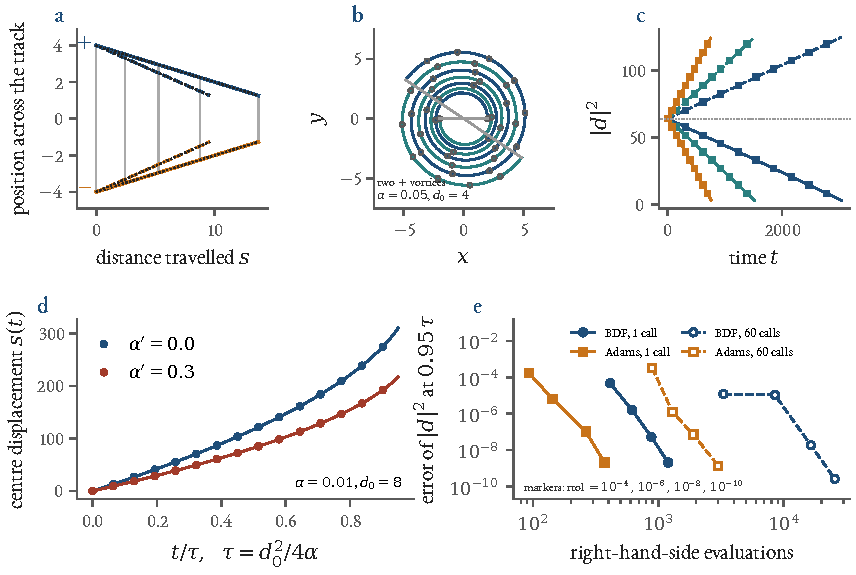
\includegraphics[width=\linewidth]{figures/ch07_dipole.pdf}
\caption[CVODE against the Lean statements on dissipative vortex pairs]{CVODE (\texttt{rusty\_sundials}) against the statements of \cref{ch07:lean}. \textbf{a}~A dipole shrinking and translating: $+$ (blue) and $-$ (orange) vortices in the frame of the track, $\alpha'=0$ (solid) and $0.3$ (dashed),
exact curves dotted, pair axis in grey at five times; $\alpha=0.2$ is ten times a thermal value, chosen so that the funnel is visible. \textbf{b}~Two $+$ vortices spiral apart ($\alpha=0.05$, $d_0=4$, $600$ time units, @@SPIRAL_TURNS@@ turns);
grey circles: closed form. \textbf{c}~$|\mathbf d|^2$ against time: dipoles (solid) fall with slope $-4\alpha$, same-sign pairs (dashed) rise with $+4\alpha$, for $\alpha=0.005,\,0.01,\,0.02$ (blue, teal, orange); filled markers $\alpha'=0$, open $\alpha'=0.3$.
\textbf{d}~Displacement of the centre of a dipole against the closed form $s=(1-\alpha')(d_0-d)/2\alpha$. \textbf{e}~Work and precision: right-hand-side evaluations against the error of $|\mathbf d|^2$ at $0.95$ of the lifetime ($\alpha=0.01$, $\alpha'=0.1$) for BDF and Adams at $\texttt{rtol}=10^{-4},\dots,10^{-10}$, in one call (filled) and in a chain of $60$ outputs (open).}
\label{ch07:fig-dipole}
\end{figure}
